\section{Laufzeitsicht}

\subsection{Anmeldung und Zugriff auf geschützte Bereiche}

Bei der Anmeldung leitet das API Gateway die Zugangsdaten an den Auth Service weiter.
Nach erfolgreicher Prüfung stellt dieser ein 60 Minuten gültiges JWT aus.

Bei geschützten Aufrufen validiert das API Gateway das Token.
Ungültige oder abgelaufene Tokens werden mit \texttt{401 Unauthorized} abgewiesen.
Andernfalls wird die Benutzer-ID ausgelesen und an den zuständigen Service weitergegeben.
Der vollständige Ablauf ist in Abbildung~\ref{fig:login} dargestellt.

\begin{figure}[htbp]
    \centering
    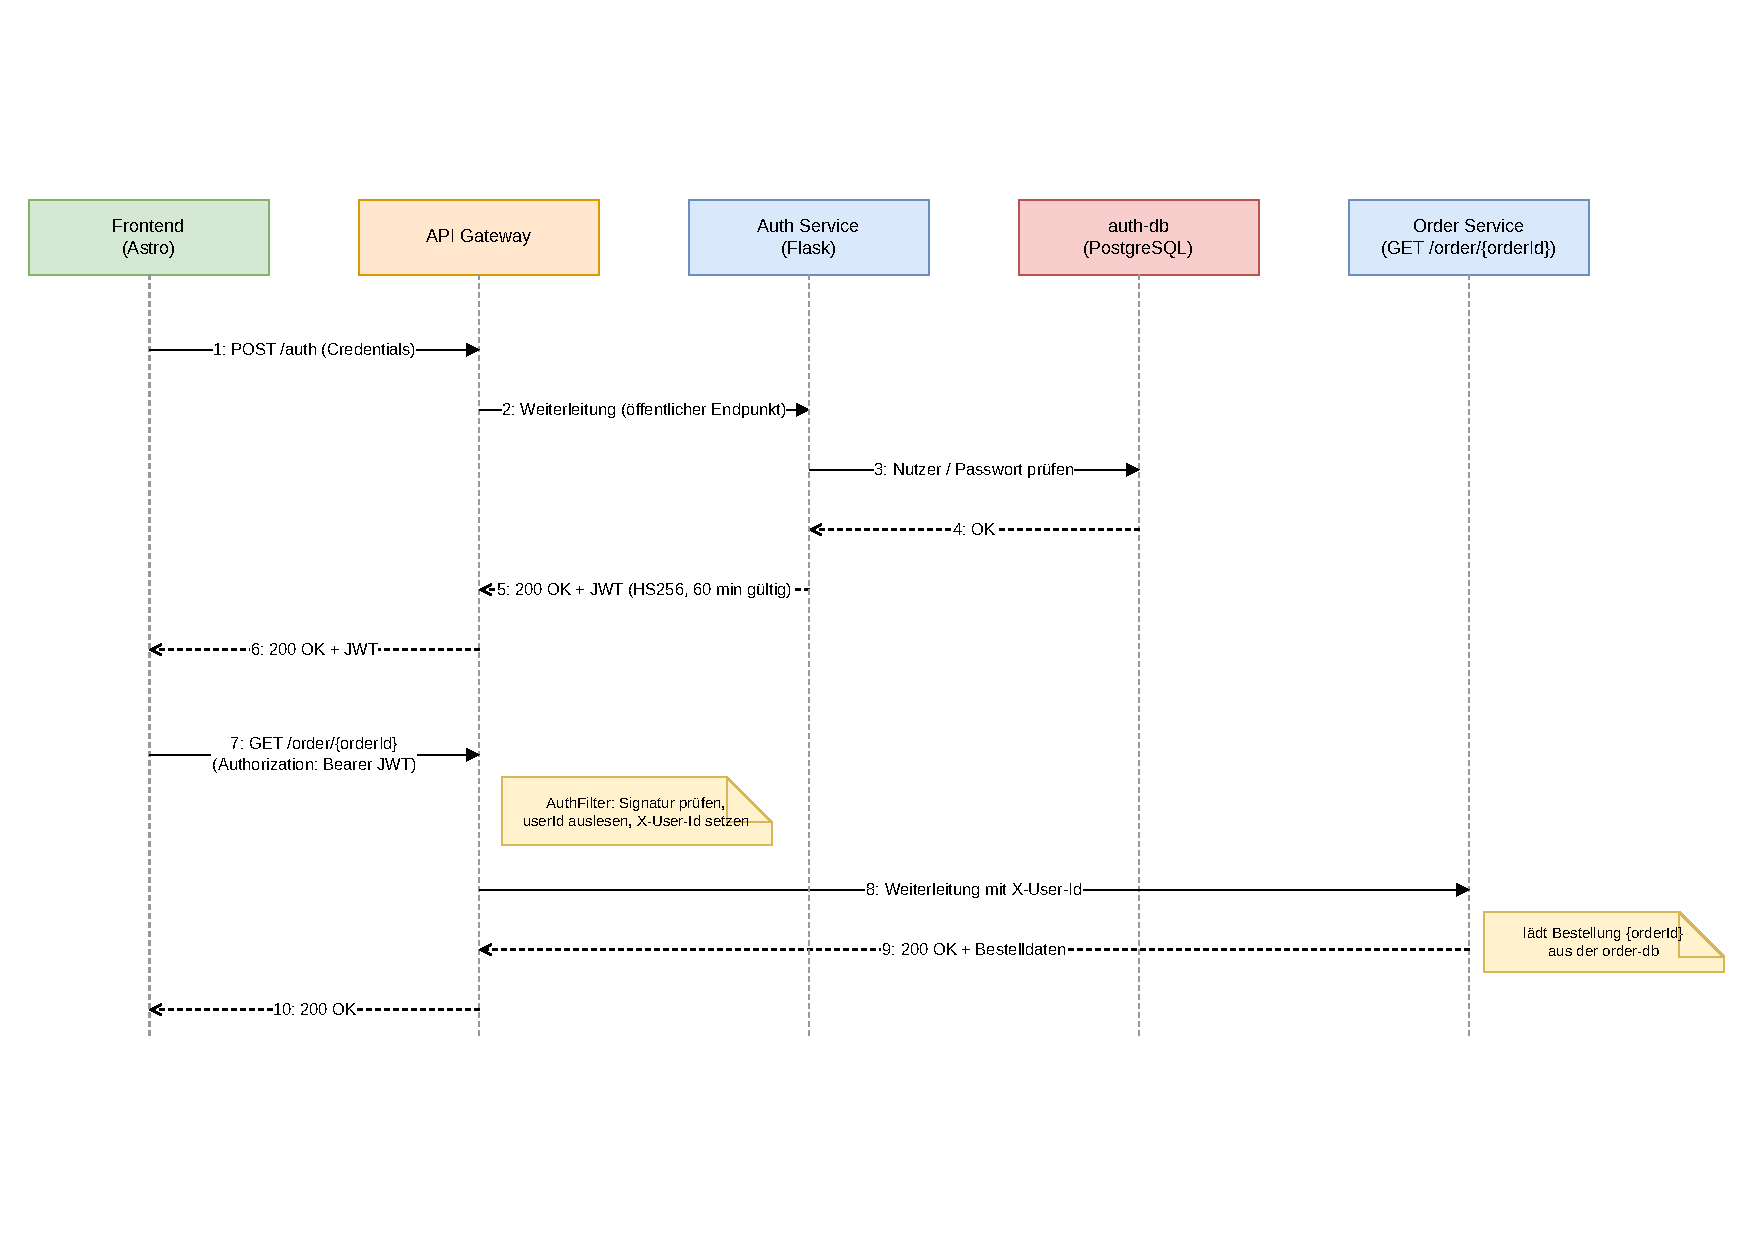
\includegraphics[width=\linewidth]{images/04-sequenz-login.pdf}
    \caption{Anmeldung und anschließender Zugriff mit Token}
    \label{fig:login}
\end{figure}

\subsection{Kauf von Artikeln}

Beim Kauf übermittelt das Frontend alle Artikel des Warenkorbs in einer Anfrage.
Der Order Service prüft beim Product Service,
ob die Artikel noch verfügbar sind und nicht dem Käufer selbst gehören.
Schlägt eine Prüfung fehl, wird der gesamte Kauf abgebrochen.

Anschließend markiert der Order Service die Artikel als verkauft.
Tritt dabei ein Fehler auf, werden bereits vorgenommene Änderungen zurückgesetzt.
Danach wird die Bestellung im Status \texttt{CREATED} gespeichert und die E-Mail-Adresse beim User Service abgerufen.

Der Order Service veröffentlicht über MQTT ein Ereignis,
das vom Email Service unabhängig verarbeitet wird.
Dadurch kann die Bestellbestätigung versendet werden,
ohne die Antwort an den Benutzer zu verzögern.

Die weiteren Statusübergänge von \texttt{CREATED} über \texttt{PAID} und
\texttt{SHIPPED} bis \texttt{DELIVERED} werden automatisch vom
Order Status Scheduler durchgeführt.
Der vollständige Ablauf ist in Abbildung~\ref{fig:buying} dargestellt.


\begin{figure}[htbp]
    \centering
    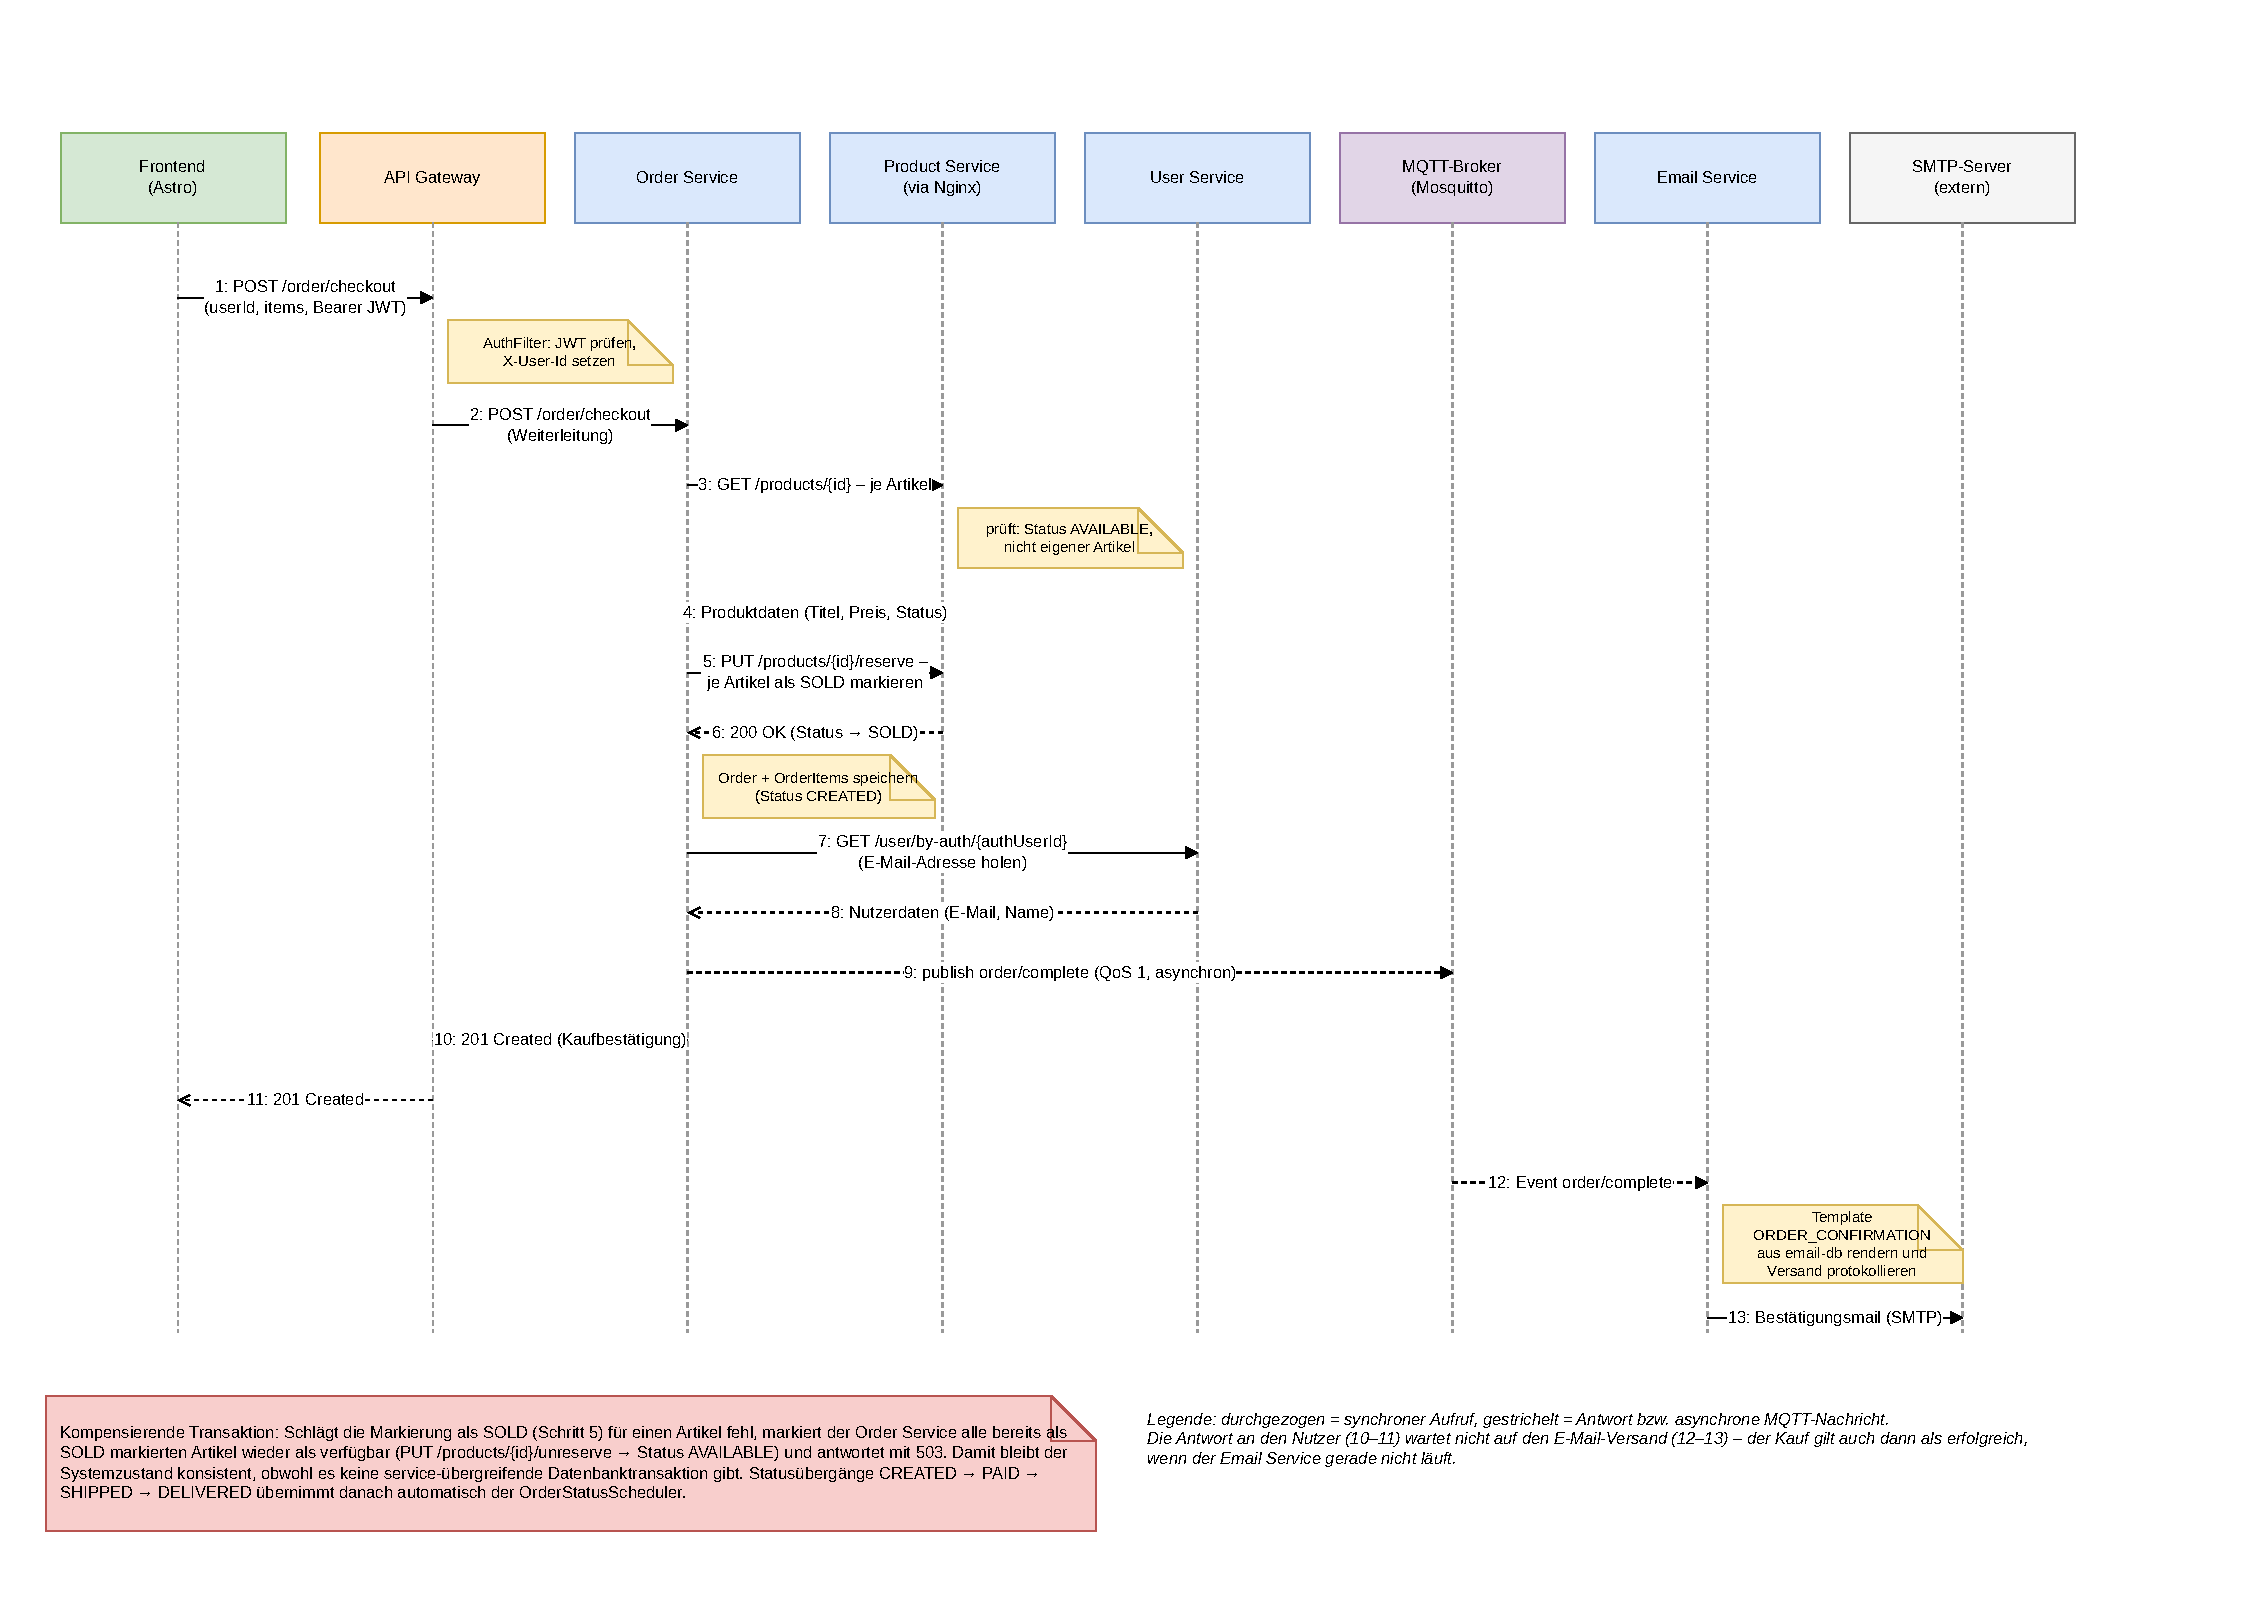
\includegraphics[width=\linewidth]{images/03-sequenz-checkout}
    \caption{Kauf von Artikeln und Versand der Bestellbestätigung}
    \label{fig:buying}
\end{figure}